\documentclass[11pt, aspectratio=169]{beamer}
\usetheme{Madrid}
\usecolortheme{default}

% Packages
\usepackage{amsmath, amssymb}
\usepackage{graphicx}
\usepackage{booktabs}
\usepackage{multirow}
\usepackage{xcolor}
\usepackage[utf8]{inputenc}
\usepackage{tikz}
\usetikzlibrary{positioning, shapes.geometric, arrows.meta}
\usepackage{booktabs}

% Title information
\title{NODLINK: Fine-Grained APT Attack Detection and Investigation}
\subtitle{NDSS 2024 Paper Review}
\author{Muhammad A'qil}
\date{\today}

% Remove navigation symbols
\setbeamertemplate{navigation symbols}{}

% Custom colors
\definecolor{critic}{RGB}{220,50,47}
\definecolor{good}{RGB}{34,139,34}

\begin{document}

% --- Slide 1: Title ---
\begin{frame}
    \titlepage
    \centering
\end{frame}

% --- Slide 2: What are APTs? ---
\begin{frame}{What are APTs?}
    \begin{block}{Advanced Persistent Threats}
        \begin{itemize}
            \item Sophisticated, long-running cyber attacks
            \item Targets: government, research, defense, critical infrastructure
            \item Multi-stage: initial compromise $\rightarrow$ lateral movement $\rightarrow$ persistence $\rightarrow$ exfiltration
        \end{itemize}
    \end{block}
    \vspace{0.5cm}
    \begin{alertblock}{SOC Challenge}
        Attack steps are buried inside massive amounts of benign system activity
    \end{alertblock}
    \begin{quote}
        \centering
        \textit{``Needle in a haystack'' — 100,000+ graph nodes, only $\sim$100 attack-relevant}
    \end{quote}
\end{frame}

% --- Slide 3: Existing Systems ---
\begin{frame}{Existing Systems}
    \begin{block}{Current Online Detection Systems Face a Trade-off}
        \begin{table}
        \centering
        \begin{tabular}{lll}
            \toprule
            \textbf{System} & \textbf{Approach} & \textbf{Problem} \\
            \midrule
            HOLMES & Rule-based & Incomplete rule sets $\rightarrow$ misses attacks \\
            UNICORN & Graph hashing & Over-approximates $\rightarrow$ 1000$\times$ false positives \\
            \bottomrule
        \end{tabular}
        \end{table}
    \end{block}
    \begin{alertblock}{Both sacrifice detection granularity for speed}
        Security analysts cannot interpret massive, noisy output graphs!
    \end{alertblock}
\end{frame}

% --- Slide 4: Steiner Tree Problem (STP) ---
\begin{frame}{Steiner Tree Problem (STP)}
    \begin{block}{Definition}
        Given:
        \begin{itemize}
            \item A graph $G = (V, E)$ with edge weights
            \item A set of \textbf{terminal nodes} $T$ (must be connected)
        \end{itemize}
        Find: The \textbf{minimum-weight subgraph} connecting all terminals
    \end{block}
\begin{figure}[htbp]
    \centering
    \begin{minipage}{0.3\linewidth}
        \centering
        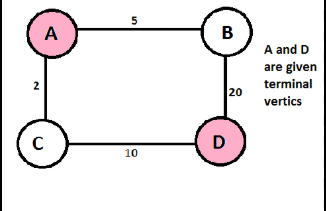
\includegraphics[width=\linewidth]{steiner2.png}
        \caption{Graph set}
        \label{fig:steiner}
    \end{minipage}
    \hfill
    \begin{minipage}{0.3\linewidth}
        \centering
        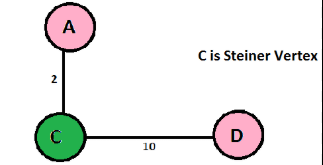
\includegraphics[width=\linewidth]{image.png}
        \caption{Steiner tree}
        \label{fig:isg}
    \end{minipage}
\end{figure}
\end{frame}

% --- Slide 5: Why STP for APT Detection? ---
\begin{frame}{Why STP for APT Detection?}
    \begin{itemize}
        \item \textbf{Terminals} = suspicious processes/nodes (identified via anomaly detection)
        \item \textbf{Steiner tree} = the minimal attack chain connecting all suspicious steps
        \item \textbf{Edge weights} = all set to 1 (simplification)
    \end{itemize}
    \begin{quote}
        \centering
        \textit{``Find the smallest subgraph that explains how all suspicious activities connect''}
    \end{quote}
    \begin{exampleblock}{Benefit}
        This provides \textbf{theoretical guarantees} on solution quality in terms of granularity.
    \end{exampleblock}
\end{frame}

% --- Slide 6: The Online STP Challenge ---
\begin{frame}{The Online STP Challenge}
    \begin{block}{Standard Online STP (Algorithm 1)}
        For each new terminal $t_i$:
        \begin{enumerate}
            \item Find shortest path to every previous terminal
            \item Pick the cheapest path
            \item Add to solution
        \end{enumerate}
        \textbf{Complexity:} $O(k \cdot \text{shortest\_path})$ — too slow for real-time
    \end{block}
    \begin{alertblock}{Problem}
        Classical STP algorithms (Kou, Mehlhorn) are \textbf{3–8400$\times$ slower} than needed for online detection
    \end{alertblock}
\end{frame}

% --- Slide 7: NODLINK Overview ---
\begin{frame}{NODLINK System Overview}
    \begin{center}
        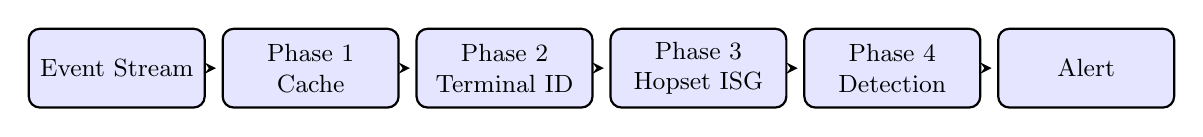
\begin{tikzpicture}[
            block/.style={rectangle, draw, thick, fill=blue!10, text width=2.0cm, align=center, minimum height=1.0cm, rounded corners, font=\small},
            arrow/.style={-stealth, thick, shorten >=2pt, shorten <=2pt}
        ]
            
            \node[block] (event) {Event Stream};
            \node[block, right=0.2cm of event] (cache) {Phase 1\\Cache};
            \node[block, right=0.2cm of cache] (terminal) {Phase 2\\Terminal ID};
            \node[block, right=0.2cm of terminal] (hopset) {Phase 3\\Hopset ISG};
            \node[block, right=0.2cm of hopset] (detect) {Phase 4\\Detection};
            \node[block, right=0.2cm of detect] (alert) {Alert};
            
            \draw[arrow] (event) -- (cache);
            \draw[arrow] (cache) -- (terminal);
            \draw[arrow] (terminal) -- (hopset);
            \draw[arrow] (hopset) -- (detect);
            \draw[arrow] (detect) -- (alert);
            
        \end{tikzpicture}
        
        \vspace{0.3cm}
        \begin{table}
            \centering
            \begin{tabular}{ll}
                \toprule
                \textbf{Phase 1} & In-Memory Cache (buffer, prioritize anomalies) \\
                \textbf{Phase 2} & Terminal ID (VAE flags suspicious processes) \\
                \textbf{Phase 3} & Hopset Construction (ISG, bounded BFS, $\theta=10$) \\
                \textbf{Phase 4} & Comprehensive Detection (merge windows, Grubb's test) \\
                \bottomrule
            \end{tabular}
        \end{table}
        
        \vspace{0.2cm}
        \textit{$\Delta = 10$ sec between Phase 1 and Phase 2}
    \end{center}
\end{frame}

% --- Slide 8: Phase 1 — In-Memory Cache ---
\begin{frame}{In-Memory Cache}
    \begin{block}{Problem}
        APT attacks can span \textbf{weeks} — cannot keep all data in memory
    \end{block}

    \begin{exampleblock}{Solution}
        \begin{itemize}
            \item Time window $\Delta = 10$ seconds
            \item Keep high-anomaly, actively evolving subgraphs in memory
            \item Evict low-energy hopsets to disk (Neo4j)
        \end{itemize}
    \end{exampleblock}

    \begin{block}{Energy Function}
        \[
        E = \epsilon^{\text{age}} \times \text{HAS}(h)
        \]
        \begin{itemize}
            \item $\epsilon = 0.8$ (decay factor)
            \item $age$ = time windows since last update, $HAS$ = hopset anomaly score
        \end{itemize}
    \end{block}
\end{frame}

% --- Slide 9: Phase 2 — Terminal Identification (VAE), Part 1 ---
\begin{frame}{Terminal Identification: Embedding}
    \begin{block}{Goal: Flag suspicious process nodes as ``terminals''}
        \textbf{Step 1: Embedding}
        \[
        V_p = w_c V_c + \sum w_{fi} V_{fi} + \sum w_{ni} V_{ni}
        \]
        \begin{itemize}
            \item $V_c$: command line (FastText embedding)
            \item $V_{fi}$: files accessed (IDF-weighted)
            \item $V_{ni}$: IP addresses connected to
        \end{itemize}
    \end{block}

\end{frame}

% --- Slide 10: Phase 2 — Terminal Identification (VAE), Part 2 ---
\begin{frame}{Terminal Identification: VAE \& Scoring}
    \begin{block}{Step 2 \& 3: VAE + Stability Score}
        \[
        AS(p) = \log\left(\frac{RE(p)}{SV(p)}\right)
        \]
        \begin{itemize}
            \item $RE(p)$ = reconstruction error from VAE
            \item $SV(p)$ = number of DBSCAN clusters for processes with same name
            \item Reduces false positives for unstable processes (e.g., web browsers)
        \end{itemize}
    \end{block}
    
    \begin{block}{Terminal Decision}
        \textbf{Threshold:} 90th percentile of historical $AS$ $\rightarrow$ flag as terminal
    \end{block}
\end{frame}

% --- Slide 10: Phase 3 — Hopset Construction (ISG) ---
\begin{frame}{Hopset Construction (ISG)}
    \begin{block}{Importance-Score-Guided algorithm}
        \textbf{Why not standard STP?} Shortest-path computation is too expensive for online use
    \end{block}
    \begin{exampleblock}{What ISG does:}
        \begin{enumerate}
            \item Start from each terminal
            \item Explore neighbors greedily by \textbf{importance score} $IV(n)$
            \item Stop after $\theta = 10$ nodes per terminal
            \item Merge overlapping explorations
        \end{enumerate}
    \end{exampleblock}
    \begin{alertblock}{Complexity: $O(\theta N)$, linear in number of nodes!}
    \end{alertblock}
\end{frame}

% --- Slide 11: ISG Algorithm ---
\begin{frame}{Importance Value (IV)}
    \begin{block}{Formula}
        \[
        IV(n) = \alpha^i \cdot (\beta \cdot AS(n) + \gamma \cdot FANOUT(n))
        \]
        \begin{table}
        \centering
        \begin{tabular}{lll}
            \toprule
            $\alpha^i$ & Distance decay ($i$ = hops from terminal) & $\alpha = 0.9$ \\
            $AS(n)$ & Anomaly score (from VAE) & Per node \\
            $FANOUT(n)$ & out\_degree / (in\_degree + 1) & Deprioritizes ``leaf'' nodes \\
            $\beta, \gamma$ & Weights & $\beta=100, \gamma=1$ \\
            \bottomrule
        \end{tabular}
        \end{table}
    \end{block}
    \begin{exampleblock}{Intuition: Explore nodes that are}
        \begin{enumerate}
            \item \textbf{Anomalous} (high AS)
            \item \textbf{Close} to known terminals (small $i$)
            \item \textbf{Not leaf nodes} (low fanout)
        \end{enumerate}
    \end{exampleblock}
\end{frame}

% --- Slide 12: Phase 4 — Comprehensive Detection ---
\begin{frame}{Comprehensive Detection}
    \begin{block}{Goal: Connect attack steps across time windows}
        \begin{enumerate}
            \item Merge current hopsets with cached hopsets (by node ID)
            \item Update hopset anomaly score: $HAS = \sum AS(n)$
            \item Run \textbf{Grubbs' test} to detect outliers
        \end{enumerate}
    \end{block}
    \begin{exampleblock}{Why Grubbs' test?}
        \begin{itemize}
            \item Non-parameterized
            \item Robust to polluted training data
            \item No manual threshold tuning
        \end{itemize}
    \end{exampleblock}
    \begin{block}{Output}
        Concise alert provenance graph ($\sim$200 nodes vs. UNICORN's 100,000+)
    \end{block}
\end{frame}

% --- Slide 13: Evaluation Overview ---
\begin{frame}{Evaluation Overview}
    \begin{block}{Datasets}
        \begin{table}
        \centering
        \begin{tabular}{llll}
            \toprule
            \textbf{Dataset} & \textbf{Type} & \textbf{Duration} & \textbf{Hosts} \\
            \midrule
            DARPA CADETS/THEIA/TRACE & Close-world & 47-264 hrs & Various \\
            Industrial Arena & Close-world & 336 hrs & 22 \\
            In-lab Arena & Close-world & 144 hrs & 5 \\
            \textbf{Open-world} & \textbf{Production} & \textbf{5 days} & \textbf{300+} \\
            \bottomrule
        \end{tabular}
        \end{table}
    \end{block}
\end{frame}

% --- Slide 14: Key Results — Accuracy ---
\begin{frame}{Accuracy}
    \begin{block}{Graph-Level Precision (Open-World)}
        \begin{table}
        \centering
        \begin{tabular}{lcc}
            \toprule
            \textbf{System} & \textbf{Precision} & \textbf{Recall} \\
            \midrule
            HOLMES & N/A (failed) & N/A \\
            UNICORN & 0.15 & 1.00 \\
            \textbf{NODLINK} & \textbf{0.35} & \textbf{1.00} \\
            \bottomrule
        \end{tabular}
        \end{table}
    \end{block}
    \begin{block}{Node-Level Precision (Open-World)}
        \begin{itemize}
            \item \textbf{NODLINK:} 0.14
            \item \textbf{UNICORN:} 0.000361 (3 orders of magnitude lower!)
            \item \textbf{HOLMES:} Failed to detect any attacks
        \end{itemize}
    \end{block}
    \begin{alertblock}{NODLINK detected \textbf{7 real attacks} that HOLMES missed entirely}
    \end{alertblock}
\end{frame}

% --- Slide 15: Key Results — Efficiency ---
\begin{frame}{Efficiency}
    \begin{block}{Throughput (events per second)}
        \begin{itemize}
            \item NODLINK: $\sim$40+ events/sec per host
            \item HOLMES: Comparable (but failed on attacks)
            \item UNICORN: Slower
            \item ProvDetector: Much slower (failed on large datasets)
        \end{itemize}
    \end{block}
\end{frame}


% --- Slide 17: Strengths ---
\begin{frame}{Strengths}
    \begin{exampleblock}{1. Novel Theoretical Framing}
        \begin{itemize}
            \item First to formalize APT detection as STP with provable bounds
            \item Subsequent work (CCLog) builds on and cites NODLINK
        \end{itemize}
    \end{exampleblock}
    \begin{exampleblock}{2. Strong Evaluation Methodology}
        \begin{itemize}
            \item First open-world evaluation for provenance-based systems
            \item 300+ real production machines (hospitals, universities, factories)
            \item 7 real attacks detected
        \end{itemize}
    \end{exampleblock}
    \begin{exampleblock}{3. Practical Impact}
        \begin{itemize}
            \item Deployed in commercial SOC (Sangfor)
            \item Reduces analyst burden: $\sim$200 nodes vs. 100,000+
            \item Open-source release + public datasets
        \end{itemize}
    \end{exampleblock}
\end{frame}

% --- Slide 18: Weaknesses ---
\begin{frame}{Weaknesses}
    \begin{alertblock}{1. ISG Algorithm Concerns}
        \begin{itemize}
            \item \textbf{Formulation mismatch:} Claims to minimize edge weight (STP) but performs no minimization
            \item \textbf{Disconnected terminals:} Behavior undefined when terminals $> \theta$ hops apart
        \end{itemize}
    \end{alertblock}
    \begin{alertblock}{2. Evaluation Limitations}
        \begin{itemize}
            \item \textbf{Ground truth bias:} Relied on Sangfor's EDR rules to filter 135k $\rightarrow$ 2k alerts
            \item \textbf{No false negative analysis:} Misses reconnaissance steps but doesn't quantify impact
        \end{itemize}
    \end{alertblock}
\end{frame}

% --- Slide 19: Possible Enhancements ---
\begin{frame}{Possible Enhancements}
    \begin{block}{1. Adaptive $\theta$}
        \begin{itemize}
            \item Gradually increase hop bound until terminals connect
            \item Log disconnected hopsets for analyst review
            \item Set $\theta$ based on graph diameter per deployment
        \end{itemize}
    \end{block}
    \begin{block}{2. Adversarial Evaluation}
        \begin{itemize}
            \item Evaluate high-IV decoy nodes exhausting $\theta$ budget
            \item Cache poisoning resilience
        \end{itemize}
    \end{block}
    \begin{block}{3. Cleaner Framing}
        \begin{itemize}
            \item Present ISG as heuristic, not STP approximation
        \end{itemize}
    \end{block}
\end{frame}

% --- Slide 21: Questions ---
\begin{frame}
    \begin{center}
        \Huge Thank You
        \vspace{1cm}
    \end{center}
\end{frame}

\end{document}